\documentclass{standalone}
\usepackage{tikz}
\usepackage{pgfplots}

\begin{document}
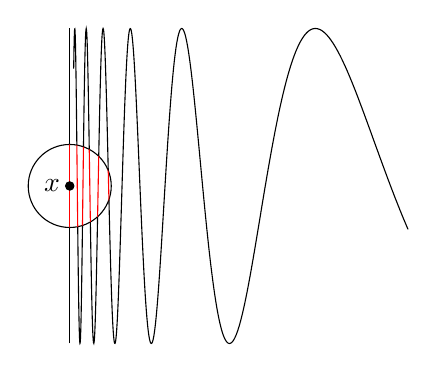
\begin{tikzpicture}[x=5cm]
\draw (0.14,-2) -- (0.14,2);
   % \draw[->] (0,-1) -- (0,1.1) node[above] {$\sin (1/x)$};
  \draw[domain=0.15:1,samples=1000, smooth] plot (\x, {2*sin((6/\x)r)});
  \filldraw[white] (0.14, 0) circle (14.7pt);
  \draw (0.14, 0) circle (15pt);
	\begin{scope}
	\clip (0.14, 0) circle (15 pt);
	\draw[red, domain=0.15:1,samples=1000, smooth] plot (\x, {2*sin((6/\x)r)});
	\draw[red] (0.14,-2) -- (0.14,2);
	\end{scope}
\filldraw (0.14, 0) circle (1.5pt) node[black, left] {$x$};
\end{tikzpicture}

\end{document}